%%%%%%%%%%%%%%%%%%%%%%%%%%%%%%%%%%%%%%%%%%%%%%%%%%%%%%%%%%%%
%%%%%%%%%%%%%%%%%%%%%%%%%%%%%%%%%%%%%%%%%%%%%%%%%%%%%%%%%%%%
%  Regret minimization and online gradient descent 
%%%%%%%%%%%%%%%%%%%%%%%%%%%%%%%%%%%%%%%%%%%%%%%%%%%%%%%%%%%%
%%%%%%%%%%%%%%%%%%%%%%%%%%%%%%%%%%%%%%%%%%%%%%%%%%%%%%%%%%%%


\chapter{
	%The conditional gradient method
	条件梯度算法
	}\label{subsec:cond_grad_intro}


%In many computational and learning scenarios the main bottleneck of optimization, both online and offline, is the computation of projections onto the underlying decision set (see \S \ref{sec:projections}). In this chapter we discuss projection-free methods in convex optimization, and some of their applications in machine learning. 
在许多计算和学习场景中,在线和离线优化的主要瓶颈是向底层决策集的投影计算(请参见 \S \ref{sec:projections})。在本章中,我们将讨论凸优化中的无投影方法,以及它们在机器学习中的一些应用。

%The motivating example throughout this chapter is the problem of matrix completion, which is a widely used and accepted model in the construction of recommendation systems. For matrix completion and related problems, projections amount to expensive linear algebraic operations and avoiding them is crucial in big data applications. 
本章中的激励示例是矩阵补全问题,这是一个在推荐系统构建中被广泛使用和接受的模型。对于矩阵补全和相关问题,投影意味着昂贵的线性代数运算,避免这些运算在大数据应用中至关重要。

%Henceforth we describe the conditional gradient algorithm, also known as the Frank-Wolfe algorithm. Afterwards, we describe problems for which linear optimization can be carried out much more efficiently than projections. We conclude with an application to exploration in reinforcement learning. 
接下来,我们将介绍条件梯度算法,也称为 Frank-Wolfe算法。然后,我们描述了一类问题,这类问题中线性优化可以比投影更有效的运行。最后,我们给出了一个在强化学习中探索的应用。

\section{
    %Review: relevant concepts from linear algebra
    回顾:线性代数相关概念
    }

%This chapter addresses rectangular matrices, which model  applications  such as recommendation systems naturally.  Consider a matrix $X \in \reals^{n \times m}$. A non-negative number $\sigma \in \reals_+$ is said to be a singular value for $X$ if there are two vectors $\uv \in \reals^n, \vv \in \reals^m$ such that 
本章讨论矩形矩阵,它自然而然地为推荐系统等应用问题建模。考虑一个矩阵 $X \in \reals^{n \times m}$。记非负数$\sigma \in \reals_+$ 是$X$的奇异值,如果有两个向量 $\uv \in \reals^n, \vv \in \reals^m$ 使得
$$  X^\top \uv  = \sigma \vv   , \quad X \vv = \sigma \uv. $$
%The vectors $\uv,\vv$ are called the left and right singular vectors respectively. The non-zero singular values are the square roots of the eigenvalues of the matrix $X X^\top$ (and $X^\top X$).  The matrix $X$ can be written as 
向量$\uv、\vv$分别称为左奇异向量和右奇异向量。非零奇异值是矩阵$X^\top$(和$X^\top X$)特征值的平方根。矩阵$X$可以写成
$$ X = U \Sigma V^\top  \ , \ U \in \reals ^{n \times \rho} \ , \ V^\top  \in \reals^{ \rho \times m} ,$$
%where $\rho = \min\{n,m\}$, the matrix $U$ is an orthogonal basis of the left singular vectors of $X$, the matrix $V$ is an orthogonal basis of right singular vectors, and $\Sigma$ is a diagonal matrix of singular values. This form is called the singular value decomposition for $X$. 
其中  $\rho = \min\{n,m\}$,矩阵 $U$是左奇异向量 $X$的正交基,矩阵 $V$是右奇异向量的正交基,$\Sigma$ 是奇异值的对角矩阵。这种形式称为 $X$ 的奇异值分解。

%The number of non-zero singular  values for $X$ is called its rank, which we denote by $k \leq \rho$. 
%The nuclear norm of $X$ is defined as the $\ell_1$ norm of its singular values, and denoted by
$X$的非零奇异值的数量称为其秩,我们用 $k \leq \rho$ 表示。
$X$的核范数定义为其奇异值的$\ell_1$范数,表示为
$$ \|X \|_* = \sum_{i=1}^\rho \sigma_i $$
%It can be shown (see exercises) that the nuclear norm is equal to the trace of the square root of the matrix times its transpose, i.e., 
可以证明(见练习),核范数等于矩阵乘以其转置的平方根的迹,即:
$$ \|X\|_* = \trace( \sqrt{ X^\top X}  ) $$
%We denote by $A \bullet B$ the inner product of two matrices as vectors in $\reals^{n \times m}$, that is
我们用 $A \bullet B$ 表示两个矩阵的内积,矩阵属于 $\reals^{n \times m}$ 空间中,即
$$A \bullet B = \sum_{i = 1}^n \sum_{j=1}^m A_{ij} B_{ij} = \trace(AB^\top) $$

\section{
    %Motivation: matrix completion and recommendation systems
    动机:矩阵补全和推荐系统
    }
\sectionmark{
    %Motivation
    动机
    }

%Media recommendations have changed significantly with the advent of the Internet and rise of online media stores. The large amounts of data collected allow for efficient clustering and accurate prediction of users' preferences for a variety of media. A well-known example is the so called ``Netflix challenge''---a competition of automated tools for recommendation from a large dataset of users' motion picture preferences. 
随着互联网的出现和在线媒体商店的兴起,媒体推荐发生了重大变化。收集的大量数据可以有效地进行聚类,并准确预测用户对各种媒体的偏好。一个著名的例子是所谓的“Netflix挑战赛”---一个从用户的电影偏好的大数据集中进行推荐自动化工具的竞赛。

%One of the most successful approaches for automated recommendation systems, as proven in the Netflix competition, is matrix completion. Perhaps the simplest version of the problem can be described as follows.  
Netflix竞赛证明,自动推荐系统最成功的方法之一是矩阵完成。也许这个问题的最简单版本可以描述如下。

%The entire dataset of user-media preference pairs is thought of as a partially-observed matrix. Thus, every person is represented by a row in the matrix, and every column represents a media item (movie). For simplicity, let us think of the observations as binary---a person either likes or dislikes a particular movie. Thus, we have a matrix $M \in \{0,1,*\}^{n \times m}$  where $n$ is the number of persons considered, $m$ is the number of movies at our library, and $0/1$ and $*$ signify ``dislike'', ``like'' and ``unknown'' respectively:
用户-媒体偏好对的整个数据集被认为是一个部分观测矩阵。因此,每个人都由矩阵中的一行表示,而每一列表示一个媒体项(电影)。为了简单起见,让我们把观察看作是二元的---一个人喜欢或不喜欢某一部电影。因此,我们有一个矩阵 $M \in \{0,1,*\}^{n \times m}$,其中 $n$是考虑的人数,$M$是我们馆藏的电影数量,$0/1$和$*$分别表示“不喜欢”、“喜欢”和“未知”:
$$ M_{ij} = \mythreecases {0}{\mbox{
    %person $i$ dislikes movie $j$
    用户 $i$ 不喜欢电影 $j$
    }}{1}{\mbox{
        %person $i$ likes movie $j$
        用户 $i$ 喜欢电影 $j$
        }}{*}{\mbox{
            %preference unknown
            偏好未知
            }} .$$ 

%The natural goal is to complete the matrix, i.e. correctly assign $0$ or $1$ to the unknown entries. As defined so far, the problem is ill-posed, since any completion would be equally good (or bad), and no restrictions have been placed on the completions.  
自然的目标是补全矩阵,即正确地将$0$或$1$分配给未知条目。根据目前的定义,这个问题是不适定的,因为任何完成都同样好(或坏),并且没有对完成设置任何限制。

%The common restriction on completions is that the ``true'' matrix has low rank. Recall that a matrix $X \in \reals^{n \times m}$ has rank $k < \rho = \min \{n,m\} $ if and only if it can be written as 
补全过程中,典型的限制是“真实”的矩阵是低秩的。注意到如果一个矩阵 $X \in \reals^{n \times m}$ 具有秩  $k \leq \rho = \min \{n,m\} $ ,则可以被写为:
$$ X = U V \ , \ U \in \reals^{n \times k} , V \in \reals^{k \times m}.  $$


%The intuitive interpretation of this property is that each entry in $M$ can be explained by only $k$ numbers. In matrix completion this means, intuitively, that there are only $k$ factors that determine a persons preference over movies, such as genre, director, actors and so on. 
这个性质直观的解释是矩阵 $M$ 中每一个元素可以由仅仅 $k$ 个数解释。
在矩阵补全中,这意味着,直观上,这里仅有 $k$ 个因素决定一个用户对电影的偏好,如 类别、导演、演员等。

%Now the simplistic matrix completion problem can be well-formulated as in the following mathematical program. Denote by $\| \cdot \|_{OB}$ the Euclidean norm only on the observed (non starred) entries of $M$, i.e., 
现在最简单的矩阵补全问题可以明确的形式化为如下的数学规划问题。使用 $\| \cdot \|_{OB}$ 表示在 $M$ 的观测元素上的欧几里得范数
$$\|X\|_{OB}^2 = \sum_{M_{ij} \neq *} X_{ij}^2.$$ 
%The mathematical program for matrix completion is given by
那么,这个矩阵补全的数学规划问题可以表述为:
\begin{align*}
& \min_{X \in \reals^{n \times m} } \frac{1}{2} \| X - M \|_{OB}^2 \\
& \text{s.t.} \quad \rank(X) \leq k. 
\end{align*}  

%Since the constraint over the rank of a matrix is non-convex, it is standard to consider a relaxation that replaces the rank constraint by the nuclear norm. %Recall that the nuclear norm of a matrix, denoted $\|M\|_*$, is the sum of its singular vectors, also equal to the trace of the square root of the matrix times its transpose, 
%$$ \| X\|_*^2 =  \left(\sum_{i=1}^{\rho} \sigma_i \right)^2 $$
由于矩阵的秩约束是非凸的,标准的处理是考虑一个核范数松弛来替换秩约束。
%It is known that the nuclear norm is a lower bound on the matrix rank if the singular values are bounded by one (see exercises). 
%Thus, we arrive at the following convex program for matrix completion: 
众所周知,如果奇异值以一为界,则核范数是矩阵秩的下界(见练习)。
因此,我们得出以下矩阵补全的凸规划问题:
\begin{align} \label{eqn:matrix-completion}
& \min_{X \in \reals^{n \times m} }  \frac{1}{2} \| X - M \|_{OB}^2 \\
& \text{s.t.} \quad \|X\|_* \leq k. \notag 
\end{align}  

%We consider algorithms to solve this convex optimization problem next. 
接下来,我们考虑解决这个凸优化问题的算法。

\section{
    %The Frank-Wolfe method
    Frank-Wolfe方法
    } 

%In this section we consider minimization of a convex function over a convex domain. 
在本节中,我们考虑凸域上凸函数的极小化。

%The conditional gradient (CG) method, or Frank-Wolfe algorithm, is a simple algorithm for minimizing a smooth convex function $f$ over a convex set $\K \subseteq \reals^n$. The appeal of the method is that it is a first order interior point method - the iterates always lie inside the convex set, and thus no projections are needed, and the update step on each iteration simply requires minimizing a linear objective over the set. The basic method is given in Algorithm \ref{alg:condgrad}.
条件梯度法(CG)或Frank Wolfe算法是一种简单的算法,用于最小化凸集 $\K \subseteq \reals^n$上的光滑凸函数 $f$。该方法的吸引力在于它是一阶内点法---迭代总是位于凸集内,因此不需要投影,每次迭代的更新步骤只需要最小化集合上的线性目标函数。基本方法在算法\ref{alg:condgrad}中给出。
\begin{algorithm}[H]
	\caption{
        %Conditional gradient
        条件梯度
        }
	\label{alg:condgrad}
	\begin{algorithmic}[1]
		%\STATE Input: step sizes $\{ \eta_t \in (0,1] , \ t \in [T]\}$, initial point $\x_1 \in \K$. 
		\STATE 输入: 步长 $\{ \eta_t \in (0,1] , \ t \in [T]\}$, initial point $\x_1 \in \K$. 
%		\STATE Let $\x_1$ be an arbitrary point in $\K$.
		\FOR{$t = 1$ to $T$}
		\STATE $\vv_{t} \gets \arg \min_{\x \in \K} \left\{\x^\top \nabla{}f(\x_t) \right\} $. \label{algstep:linearopt}
		\STATE $\x_{t+1} \gets \x_t + \eta_t(\vv_t - \x_t)$.
		\ENDFOR
	\end{algorithmic}
\end{algorithm}

%Note that in the CG method, the update to the iterate $\x_t$ may be not be in the direction of the gradient, as $\vv_t$ is the result of a linear optimization procedure in the direction of the negative gradient. This is depicted in Figure \ref{fig:OFW}. 
注意,在CG方法中,迭代$\x_t$的更新可能不在梯度方向上,因为$\vv_t$是负梯度方向上线性优化过程的结果。如图\ref{fig:OFW}所示。

\begin{figure}[h!]
\begin{center}
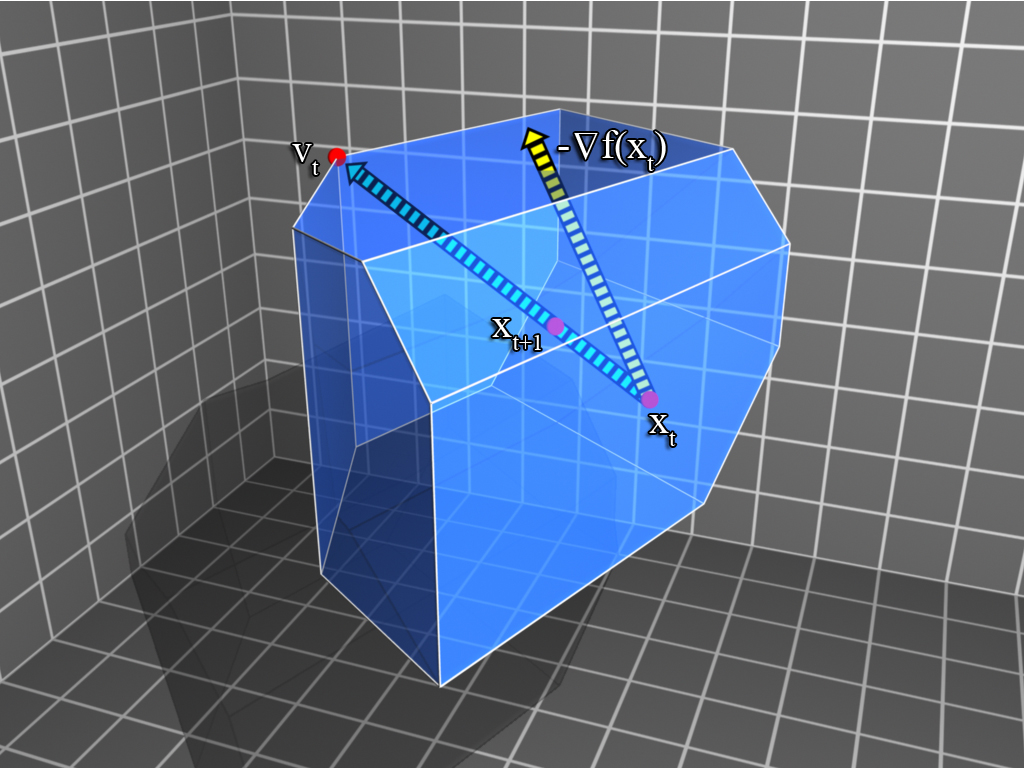
\includegraphics[width=3.5in]{figs/fig_fw2}
\end{center}
\caption{
    %Direction of progression of the conditional gradient algorithm. 
    条件梯度算法的前进方向。
    \label{fig:OFW}}
\end{figure}

%The following theorem gives an essentially tight performance guarantee of this algorithm over smooth functions. Recall our notation from Chapter \ref{chap:opt}: $\x^\star$ denotes the global minimizer of $f$ over $\K$, $D$ denotes the diameter of the set $\K$, and $h_t = f(\x_t) - f(\x^\star)$  denotes the suboptimality of the objective value in iteration $t$.
下面的定理为该算法在光滑函数上提供了严格的性能保证。回想一下我们在第\ref{chap:opt}章中的符号:$\x^\star$表示 $f$在 $\K$上的全局极小值,$D$表示集合 $\K$的直径,$h_t = f(\x_t) - f(\x^\star)$ 表示迭代 $t$中目标值的次优解。
\begin{theorem} \label{thm:offlineFW}
%The CG algorithm applied to $\beta$-smooth functions with step sizes $\eta_t =  \min\{\frac{2H}{t},1\}$, for $H \geq \max\{1,h_1\} $,  attains the following convergence guarantee:
CG算法应用于$\beta$光滑函数,取步长为 $\eta_t =  \min\{\frac{2H}{t},1\}$,对于 $H \geq \max\{1,h_1\} $,可获得以下收敛保证:
$$ h_t \leq \frac{2 \beta H D^2 }{t} $$
\end{theorem}
\begin{proof}[证明]
%As done before in this manuscript, we denote $\nabla_t = \nabla f(\x_t)$, and also denote $H \geq \max \{h_1,1\}$, such that $\eta_t = \min\{ \frac{2 H}{t},1\}$.  For any set of step sizes, we have
与本书之前一样,我们记 $\nabla_t = \nabla f(\x_t)$,记 $H \geq \max \{h_1,1\}$,使得 $\eta_t = \min\{ \frac{2 H}{t},1\}$。对于任何一组步长,我们都有
\begin{align}\label{old_fw_anal}
	&  f(\x_{t+1}) - f(\x^\star) 
	= f(\x_t + \eta_t(\vv_t - \x_t)) - f(\x^\star) \notag \\
	&\leq  f(\x_t) - f(\x^\star) + \eta_t(\vv_t-\x_t)^{\top}\nabla_t + \eta_t^2 \frac{\beta}{2}\Vert{\vv_t-\x_t}\Vert^2 &  \textrm{
        %$\beta$-smoothness
        $\beta$-平滑
        } \nonumber \\
	&\leq  f(\x_t) - f(\x^\star) + \eta_t(\x^\star-\x_t)^{\top}\nabla_t + \eta_t^2 \frac{\beta}{2}\Vert{\vv_t-\x_t}\Vert^2 &  \textrm{
        %$\vv_t$ optimality
        $\vv_t$ 优化解
        } \nonumber \\
	&\leq  f(\x_t) - f(\x^\star) + \eta_t(f(\x^\star)-f(\x_t)) + \eta_t^2 \frac{\beta}{2}\Vert{\vv_t-\x_t}\Vert^2 & \textrm{
        %convexity of $f$
        $f$ 的凸性质
        } \nonumber \\
	&\leq  (1-\eta_t)(f(\x_t)-f(\x^\star)) + \frac{\eta_t^2\beta}{2} D^2. 
\end{align}
%We reached the recursion $ h_{t+1} \leq (1- \eta_t) h_t + \eta_t^2\frac{  \beta D^2}{2} $, and by induction,
我得到递归 $ h_{t+1} \leq (1- \eta_t) h_t + \eta_t^2\frac{  \beta D^2}{2} $,通过归纳:
\begin{align*}
 h_{t+1} & \leq (1- \eta_t) h_t + \eta_t^2 \frac{\beta D^2}{2}  \\
 & \leq (1- \eta_t) \frac{2  \beta H D ^2 }{ t} + \eta_t^2 \frac{ \beta  D^2}{2} & \mbox{
     %induction hypothesis
     归纳假设
     }\\
 & \leq (1- \frac{2 H}{ t}) \frac{2  \beta H D^2}{t} + \frac{4 H^2}{  t^2} \frac{\beta D^2 }{2}& \mbox{
     %value of $\eta_t$
     $\eta_t$ 的值
     }\\
 & = \frac{2  \beta H D^2 }{t} -  \frac{2 H^2 \beta D^2 }{ t^2 } \\
 & \leq \frac{2  \beta H D^2 }{t} (1 - \frac{1}{t} ) & \mbox{
     %since $H \geq 1$
     因为$H \geq 1$
     } \\
 & \leq \frac{2  \beta H D^2 }{t+1 }.  & \mbox{$\frac{t-1}{t} \leq \frac{t}{t+1} $ } \\
 \end{align*}

\end{proof}


\section{
    %Projections vs. linear optimization
    投影 vs. 线性优化
    }

%The conditional gradient (Frank-Wolfe) algorithm described before does not resort to projections, but rather computes a linear optimization problem of the form
前面描述的条件梯度(Frank Wolfe)算法不依赖于投影,而是计算如下形式的线性优化问题
\begin{equation} \label{eqn:linopt}
 \arg \min_{\x \in \K} \left\{\x^\top \uv \right\}. 
\end{equation}
%When is the CG method computationally preferable?  The overall computational complexity of an iterative optimization algorithm is the product of the number of iterations and the computational cost per iteration. The CG method does not converge as well as the most efficient gradient descent algorithms, meaning it requires more iterations to produce a solution of a comparable level of accuracy. However, for many interesting scenarios the computational cost of a linear optimization step \eqref{eqn:linopt} is {\em significantly} lower than that of a projection step. 
什么时候CG方法在计算上更可取?迭代优化算法的总体计算复杂度是迭代次数和每次迭代的计算成本的乘积。CG方法的收敛性不如最有效的梯度下降算法,这意味着它需要更多的迭代才能产生具有同等精度的解决方案。然而,对于许多有趣的场景,线性优化步骤的计算成本\eqref{eqn:linopt}明显低于投影步骤。

%The latter argument is especially relevant in online convex optimization: where as in offline optimization the CG algorithm behaves polynomially in $\eps$ as compared to logarithmically for well-conditioned problems, for OCO such differences are impossible - we have seen in previous chapters that the regret is bounded by square root in the number of iterations. 
后一种观点在在线凸优化中尤其重要:在离线优化中,CG算法在$\eps$中表现为多项式,而在条件良好的问题中,CG算法表现为对数,对于OCO,这种差异是不可能的---我们在前几章中已经看到,遗憾损失的范围是迭代次数的平方根。

%Let us  point out several examples of problems for which we have very efficient linear optimization algorithms, whereas our state-of-the-art algorithms for computing projections  are significantly slower. 
让我们列举几个问题的例子,对于这些问题,我们有非常有效的线性优化算法,而用于计算投影的最先进算法要慢得多。

\paragraph*{
    %Recommendation systems and matrix prediction.
    推荐系统与矩阵补全
    }

%In the example pointed out in the preceding section of matrix completion, known methods for projection onto the spectahedron, or more generally the bounded  nuclear-norm ball, require singular value decompositions, which  take superlinear time via our best known methods. In contrast, the CG method requires maximal eigenvector computations which can be carried out in linear time via the power method (or the more sophisticated Lanczos algorithm). 
在前面的矩阵补全部分指出的例子中,投影到 spectahedron (xx多面体?),或者更一般地说,投影到有界核范数球,的已知方法需要奇异值分解,通过我们最著名的方法,这需要超线性时间。相比之下,CG方法只需要最大特征向量计算,这可以通过幂法(或更复杂的Lanczos算法)在线性时间内进行。

\paragraph*{
    %Network routing and convex graph problems.
    网络路由与凸图问题
    }

%Various routing and graph problems can be modeled as convex optimization problems over a convex set called the flow polytope. 
各种路由和图问题都可以建模为一个称为流多面体的凸集上的凸优化问题。

%Consider  a directed acyclic graph with $m$ edges, a source node marked $s$ and a target node marked $t$. Every path from $s$  to $t$ in the graph can be represented by its identifying vector, that is a vector in $\lbrace{0,1}\rbrace^m$ in which the entries that are set to 1 correspond to edges of the path. The flow polytope of the graph is the convex hull of all such identifying vectors  of the simple paths from $s$ to $t$. This polytope is also exactly the set of all unit $s$--$t$ flows in the graph if we assume that each edge has a unit flow capacity (a flow is represented here as a vector in $\mathbb{R}^m$ in which each entry is the amount of flow through the corresponding edge). 
考虑一个带 $m$边的有向无环图,一个标记为 $s$的源节点和一个标记为 $t$的目标节点。图中从 $s$到$t$的每条路径都可以用其标识向量表示,即 $\lbrace{0,1}\rbrace^m$ 中的向量,其中设置为 1的条目对应于路径的边。图的流多面体是从$s$到$t$的简单路径的所有此类识别向量的凸包。如果我们假设每一条边都有一个单位流容量(一个流在这里表示为 $\mathbb{R}^m$中的向量,其中每个条目都是通过相应边的流量),那么这个多面体也是图中所有单位$s$--$t$流的集合。

%Since the flow polytope is just the convex hull of $s$--$t$ paths in the graph, minimizing a linear objective over it amounts to finding a minimum weight path given weights for the edges. For the shortest path problem we have  very efficient combinatorial optimization algorithms, namely Dijkstra's algorithm. 
由于流多面体只是图中 $s$--$t$路径的凸包,因此最小化其上的线性目标相当于找到给定边权重的最小权重路径。对于最短路径问题,我们有非常有效的组合优化算法,即Dijkstra算法。

%Thus, applying the CG algorithm to solve {\bf any} convex optimization problem over the flow polytope will only require iterative shortest path computations. 
因此,应用CG算法求解流多面体上的{\bf 任意}凸优化问题只需要迭代最短路径计算。


\paragraph*{
    %Ranking and permutations. 
    排序和置换
    }

%A common way to represent a permutation or ordering is by a permutation matrix. Such are square matrices over $\{0,1\}^{n \times n}$ that contain exactly one $1$ entry in each row and column.  
表示置换或排序的常用方法是通过置换矩阵。这样的矩阵是 $\{0,1\}^{n \times n}$上的方阵,每行和每列正好包含一个$1$条目。

%Doubly-stochastic matrices are square, real-valued matrices with non-negative entries, in which the sum of entries of each row and each column amounts to 1. The polytope that defines all doubly-stochastic matrices is called the Birkhoff-von Neumann polytope. 
%The Birkhoff-von Neumann theorem states that this polytope is the convex hull of exactly all $n\times{n}$ permutation matrices. 
双随机矩阵是具有非负项的平方实值矩阵,其中每行和每列的项之和为1。定义所有双随机矩阵的多面体称为 Birkhoff-von Neumann多面体。
Birkhoff-von Neumann 定理指出,这个多面体是所有  $n\times{n}$置换矩阵的凸包。

%Since a permutation matrix corresponds to a perfect matching in a fully connected bipartite graph, linear minimization over this polytope corresponds to finding a minimum weight perfect matching in a bipartite graph. 
由于一个置换矩阵对应于一个完全连通的二部图中的一个完美匹配,所以这个多面体上的线性极小化对应于在一个二部图中找到一个最小权重的完美匹配。

%Consider a convex optimization problem over the Birkhoff-von Neumann polytope. The CG algorithm will iteratively solve a linear optimization problem over the BVN polytope, thus iteratively solving a minimum weight perfect matching in a bipartite graph problem, which is a well-studied combinatorial optimization problem for which we know of efficient algorithms. In contrast, other gradient based methods will require projections, which are quadratic optimization problems over the BVN polytope.
考虑Birkhoff-von Neumann多面体上的一个凸优化问题。CG算法将迭代求解BVN多面体上的线性优化问题,从而迭代求解二部图问题中的最小权重完美匹配问题,这是一个研究得很好的组合优化问题,我们知道它的有效算法。相比之下,其他基于梯度的方法将需要投影操作,这是BVN多面体上的二次优化问题。

\paragraph*{
    %Matroid polytopes.
    拟阵多面体
    }

%A matroid is pair $(E,I)$ where $E$ is a set of elements and $I$ is a set of subsets of $E$ called the independent sets which satisfy various interesting proprieties that resemble the concept of linear independence in vector spaces. 
%Matroids have been studied extensively in combinatorial optimization and a key example of a matroid is the graphical matroid in which the set $E$ is the set of edges of a given graph and the set $I$ is the set of all subsets of $E$ which are cycle-free. In this case, $I$ contains all the spanning trees of the graph. A subset $S\in{I}$ could be represented by its identifying vector which lies in $\lbrace{0,1}\rbrace^{\vert{E}\vert}$ which also gives rise to the matroid polytope which is just the convex hull of all identifying vectors of sets in $I$. It can be shown that some matroid polytopes are defined by exponentially many linear inequalities (exponential in $\vert{E}\vert$), which makes optimization over them difficult. 
拟阵是 $(E,I)$ 对,其中 $E$是一组元素,$I$是$E$的子集,称为独立集,满足各种有趣的性质,类似于向量空间中线性独立的概念。
拟阵在组合优化中得到了广泛的研究,其中的一个关键例子是图拟阵,其中集合 $E$是给定图的边集合,集合 $I$是集合$E$的所有无环子集。在这个例子中,$I$包含图的所有生成树。一个子集$S\in{I}$可以用它的识别向量来表示,它位于$\lbrace{0,1}\rbrace^{\vert{E}\vert}$中,这也产生了拟阵多面体,它只是$I$中所有识别向量的凸包。可以证明,一些拟阵多面体是由指数级多的线性不等式(关于$\vert{E}\vert$ 的指数)定义的,这使得对它们的优化变得困难。

%On the other hand, linear optimization over matroid polytopes is easy using a simple greedy procedure which runs in nearly linear time. Thus, the CG method serves as an efficient algorithm to solve any convex optimization problem over matroids iteratively using only a simple greedy procedure. 
另一方面,拟阵多面体上的线性优化很容易使用一个简单的贪心过程,该过程在几乎线性的时间内运行。因此,CG方法可以作为一种有效的算法,只需使用一个简单的贪心过程就可以迭代地解决拟阵上的任何凸优化问题。


\newpage
\section{
    %Exercises
    练习题
    }

\begin{enumerate}

\item
%Prove that if the singular values are smaller than or equal to one, then the nuclear norm is a lower bound on the rank, i.e., show $$ \rank(X) \geq \|X\|_* .$$ 
证明:如果奇异值小于或等于1,则核范数是秩的下界,即 $$ \rank(X) \geq \|X\|_* .$$

\item
%Prove that the trace  is related to the nuclear norm via
证明:迹与核规范有关,形式为:
$$ \| X \|_* = \trace( \sqrt{X X^\top} ) = \trace( \sqrt{ X^\top X} ) .$$

\item
%Show that maximizing a linear function over the spectahedron is equivalent to a maximal eigenvector computation. That is, show that the following mathematical program:
证明:最大化spectahedron上的线性函数等价于最大特征向量计算。也就是说,证明以下数学规划:
\begin{align*} 
& \min  X \bullet C  \\
& X \in S_d = \{ X \in \reals^{d \times d} \ , \ X \succcurlyeq 0 \ , \ \trace(X)  \leq 1 \} ,
\end{align*}  
%is equivalent to the  following: 
等价于:
\begin{align*} 
& \min_{\x \in \reals^d}  \x^\top C \x  \\
& \mbox{s.t.  }   \|\x\|_2  \leq 1 .
\end{align*}  


\item

%Download the MovieLens dataset from the web. Implement an online recommendation system based on the matrix completion model: implement the OCG and OGD algorithms for matrix completion. Benchmark your results. 
从网上下载 MovieLens数据集。实现基于矩阵补全模型的在线推荐系统:实现用于矩阵补全的OCG和OGD算法。测试你的结果。

\end{enumerate}





\newpage
\section{
    %Bibliographic Remarks
    书目说明
    }

%The matrix completion model has been extremely popular since its inception in the context of recommendation systems \cite{SrebroThesis,Rennie:2005,salakhutdinov:collaborative,lee:practical,CandesR09,ShamirS11}.
矩阵补全模型自诞生以来,在推荐系统的背景下一直非常流行,例如\cite{SrebroThesis,Rennie:2005,salakhutdinov:collaborative,lee:practical,CandesR09,ShamirS11}。

%The conditional gradient algorithm was devised in the seminal paper by Frank and Wolfe \cite{FrankWolfe}. Due to the applicability of the FW algorithm to large-scale constrained problems, it has been a method of choice in recent machine learning applications, to name a few: 
条件梯度算法是由 Frank 和 Wolfe \cite{FrankWolfe} 在开创性的论文中设计的。由于FW算法对大规模约束问题的适用性,它已成为最近机器学习应用中的一种选择方法,仅举几例:
\cite{Jaggi10, Jaggi13a, Jaggi13b, Dudik12a, Dudik12b, Hazan12, ShalevShwartz11, Bach12, Tewari11, Garber11, Garber13, Florina14}.

%The online conditional gradient algorithm is due to \cite{Hazan12}. An optimal regret algorithm, attaining the $O(\sqrt{T})$ bound, for the special case of polyhedral sets was devised in \cite{Garber13}.
在线条件梯度算法的提出归功于\cite{Hazan12}。在\cite{Garber13}中,针对多面体集的特殊情况,设计了一个最佳遗憾算法,即达到 $O(\sqrt{T})$界。
